This project involves creating the game of "Othello" (also known as "Reversi").

Othello is a two-player game. Players take it in turns to place coloured
counters on a board. If a player arranges for their own colour counters
to be at both ends of a row of counters (horizontal, vertical or diagonal),
all the counters in between change to that colour. The object of the game 
is to turn all the counters into your own colour.

Start by constructing an 8x8 game board. When you click on a cell, a
coloured spot should be drawn in the cell. Arrange it so that the colour
of the spot alternates with each click.

You will probably want to represent the game board in an array, with each
cell storing whether it is empty or has a counter in it. Players are only 
allowed to place counters next to other counters, so you will need to add this
restriction. At the start of the game, there are four counters on the board:

\begin{center}
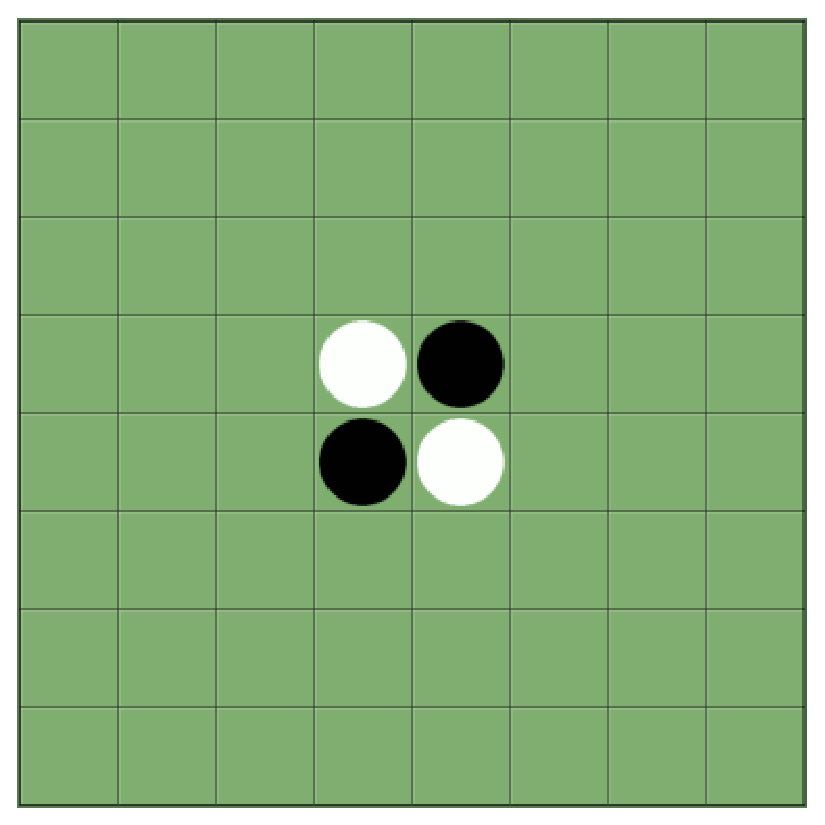
\includegraphics[scale=0.6,angle=0]{screenshots/othello}
\end{center}

The game ends when all the counters are one colour, or there are no spare
spaces to add counters.

\subsection{Extension}

Add networking to the game, so that the two players can be on different
computers. See the extension of the Paint program for some suggestions.

